\documentclass{report}

\input{~/latex/template/preamble.tex}
\input{~/latex/template/macros.tex}

\title{\Huge{Chapter 8}}
\author{\huge{Matt Warner}}
\date{\huge{}}
\pagestyle{fancy}
\fancyhf{}
\rhead{}
\lhead{\leftmark}
\cfoot{\thepage}
% \usepackage[default]{sourcecodepro} \usepackage[T1]{fontenc}

\pgfpagesdeclarelayout{boxed}
{
  \edef\pgfpageoptionborder{0pt}
}
{
  \pgfpagesphysicalpageoptions
  {%
    logical pages=1,%
  }
  \pgfpageslogicalpageoptions{1}
  {
    border code=\pgfsetlinewidth{1.5pt}\pgfstroke,%
    border shrink=\pgfpageoptionborder,%
    resized width=.95\pgfphysicalwidth,%
    resized height=.95\pgfphysicalheight,%
    center=\pgfpoint{.5\pgfphysicalwidth}{.5\pgfphysicalheight}%
  }%
}

\pgfpagesuselayout{boxed}

\begin{document}
  \maketitle
  \section*{Chapter 8 - Confidence Intervals Based on a Single Sample}
    \textbf{Satistical inference - }using a sample statistic (e.g. $\overline{x}$ = sample mean) to make some statement or some conclusion about a population parameter (e.g. $\mu$ = population mean) There are two types.
    \begin{itemize}
      \item \textbf{Confidence interval} 
        \begin{itemize}[label=$\circ$]
          \item Uses a sample statistic to \textit{estimate} the unknown value of a parameter.
          \item We write the estimate in the form of an interval that we belive captures the actual or true parameter value.
          \item The confidence interval has a specified level of confidence.
        \end{itemize}
      \item \textbf{Hypothesis Test} (or significance test)
    \end{itemize}
    \bigbreak \noindent
    \subsection*{Section 8.2 - A Confidence Interval for a Population Mean when $\sigma$ is Known}
    \begin{itemize}
      \item Provided 
        \begin{itemize}[label=$\circ$]
          \item Underlying population has a normal distribution or $n$ is large $ \left(n \ge 30\right)$
          \item $\sigma$ (\underline{population} standard deviation) has a \underline{known value}
        \end{itemize}
      \item A $100(1 - a)\%$ confidence interval to estimate $\mu$ is: 
        $$ \overline{x}\pm \left(Z_{\frac{a}{z}}\cdot \frac{\sigma}{\sqrt{n}}\right)$$
      \item The \textbf{\underline{critical value}} $ \left(Z_{a}{z}\right)$ is chosen based on the \textbf{\underline{level of confidence}}
        \vspace{1mm}

        \subitem \hspace{-7mm}$\pm{Z\frac{a}{z}}$ = values from a standard normal distribution that capture the middle $100(1-a)\%$
      \item Simplified form
        \begin{itemize}[label=$\circ$]
          \item estimate $\pm${ margin of error}
          \item \textbf{margin of error} = (critical value x \textbf{standard error of $\overline{\mathbf{x}}$})
        \end{itemize}
    \end{itemize}
\q
\textbf{An administrator at a large university wants to estimate $\mu$, the mean GPA of all students on campus. A random sample of $ n = 50$ students is selected and the GPA of each student is recorded. The resulting mean is $\overline{x} = 2.60$. Assume that the GPAs in the population are normally distributed with $\sigma = 0.75$}
\bigbreak \noindent \bigbreak \noindent
\textbf{Problem 1. Calculate a 95\% confidence interval}
\bigbreak \noindent
\textit{\textbf{its asking for 95\%, so our tails are}}

$$ \alpha = .05 \rightarrow \dfrac{\alpha}{2} = 0.25$$
\textit{\textbf{our z scores are then}}

$$ \pm 1.96$$
\textit{\textbf{So, using the formula}}
$$ \overline{x}\pm \left(Z_{\frac{a}{z}}\cdot \frac{\sigma}{\sqrt{n}}\right)$$
\textit{\textbf{We have}}
$$ 2.60\pm(1.96\cdot\dfrac{.75}{\sqrt{50}})$$
\textit{\textbf{our confidence intervals are then}}

$$ 2.60 \pm .21$$

$$ = 2.39, 2.81$$
\bigbreak \noindent \bigbreak \noindent
\hrule
\bigbreak \noindent
\textbf{Problem 2. Calculate a 90\% confidence interval to estimate $\mu$}
\bigbreak \noindent
\textit{\textbf{If its asking for 90\% are tails are}}

$$ 0.05$$
\textit{\textbf{Our z scores are then}}

$$\pm{1.6499}$$
\textit{\textbf{So, using the formula}}

$$ \overline{x}\pm \left(Z_{\frac{a}{z}}\cdot \frac{\sigma}{\sqrt{n}}\right)$$
\textit{\textbf{We have}}

$$ 2.60\pm(1.6449 \cdot\dfrac{.75}{\sqrt{50}})$$
\textit{\textbf{So, our confidence intervals are}}
$$ 2.60\pm{.17}$$
$$ = 2.43, 2.77$$
\bigbreak \noindent \bigbreak \noindent
\hrule
\bigbreak \noindent
\textbf{Problem 3. Calculate a 99\% confidence interval to estimate $\mu$}
\bigbreak \noindent
\textit{\textbf{99\% means are tails are}}

$$.005$$
\textit{\textbf{our z scores would then be}}

$$\pm{2.5758}$$
\textit{\textbf{So}}

$$2.60\pm(2.5758\cdot\dfrac{.75}{\sqrt{50}})$$
\textit{\textbf{So, our confidence intervals are}}

$$ 2.60\pm{.27}$$
$$ 2.33, 2.87$$

\pagebreak
\subsection*{The effect of choosing the confidence level and sample size}
The confidence level (90\%, 95\%, 99\% etc. ) and the sample size ($n$) are chosen by the statistician or researcher. It is important to understand how these choices affect the overall length of the confidence interval.
\bigbreak \noindent
\begin{itemize}
  \item If the confidence level \textbf{increases} then the interval gets \textbf{wider} and \textbf{less} precise
  \item If the confidence level \textbf{decreases}, then the interval gets \textbf{narrower} and \textbf{more }precise
  \item If the sample size $n$ \textbf{increases} then the interval gets \textbf{narrower} and \textbf{more} precise
  \item If the sample size $n$ \textbf{decreases}, then the interval gets \textbf{wider} and \textbf{less} precise
\end{itemize}
\bigbreak \noindent
\q
Which confidence interval would be longer and which would be shorter?
\bigbreak \noindent
(a) 90\% confidence and $n$ = 50 
\vspace{1mm}

\hspace{-4mm}95\% confidence and $n$ = 50
\vspace{1.5mm}

\sol
\vspace{1mm}

\noindent 95\% confidence interval would be longer than 90\%

\bigbreak \noindent
(b) 95\% confidence and $n$ = 50
\vspace{1mm}

\hspace{-5mm} 95\% confidence and $n$ = 100
\vspace{1.5mm}

\sol
\vspace{1.5mm}

\noindent 95\% confidence and $n$ = 50 would be longer
\bigbreak \noindent
\subsection*{Meaning of confidence}
In the previous example
\begin{itemize}
  \item $\mu$ (= mean GPA of the entire campus) is \textbf{unknown} but it has a \textbf{fixed value}
  \item After getting the sample and making our calculation, our 95\% confidence interval is also \textbf{fixed} with endpoints 2.39 to 2.81
  \item But, if we took another sample we would likely get a different $\bar{x}$ and \textbf{different} endpoints than before, and we would still state that we are confident the new interval captures $\mu$.
\end{itemize}
\bigbreak \noindent
\subsection*{Sample size calculation}
\textbf{Before} the sample is picked
\begin{itemize}
  \item we specify the desired 
    \begin{itemize}[label=$\circ$]
      \item confidence level 
      \item bound for the margin of error (B)
    \end{itemize}
  \item we ask: What size sample is needed?
    $$ n = \left(\dfrac{\sigma \cdot Z_{\frac{a}{2}}}{B}\right)^2$$
\end{itemize}
\nt{
  \textbf{ALways} round $n$ up to a whole number
}
\section*{8-3 A Confidence Interval for a Population Mean when $\sigma$ is Unknown}
\begin{itemize}
  \item Provided 
    \begin{itemize}[label=$\circ$]
      \item Underlying population has a normal distribution 
      \item $\sigma$ (population standard deviation) has an \textbf{unknown value}
      \item $s$ (sample standard deviation) has a \textbf{known value}
    \end{itemize}
  \item A 100(1 - a)\% confidence interval to estimate $\mu$ is
    $$ \bar{x} \pm \left(t_{\frac{a}{z}}\cdot \frac{s}{\sqrt{n}}\right)$$
  \item $\pm{t\frac{a}{z}}$ = critical values from a \textbf{t distribution} (with \textbf{degree of freedom} $df = n-1$) that capture the middle 100(1 - $a$)\%
\end{itemize}
\bigbreak \noindent
\subsection*{Facts about the t distribution}
\begin{itemize}
  \item It is described by a symmetric, bell-shaped curve that is centered at 0. 
  \item There are many t distributions. Each is identified by giving its degree of freedom ($df$).
  \item It is wider and has more spread than the standard normal distribution
  \item As the $df$ increases the t distribution looks more like the standard normal distribution.
\end{itemize}
\begin{figure}[ht]
\centering
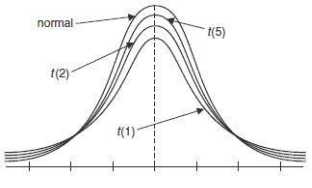
\includegraphics[width=0.5\textwidth]{ /home/mattw/niu/Stat200/latexdocs/figures/tdis.png }
\end{figure}
\q In each of the following, find the appropriate t critical value for use in constructing a condidence interval
\bigbreak \noindent
\textbf{Problem 1. } n = 10, 90\% confident
$$ df = n - 1$$
$$ df = 9$$
$$t_{.05,9} = 1.8331$$
\bigbreak \noindent \bigbreak \noindent
\textbf{Problem 2.} n = 15, 95\% confidence
$$ df = 14$$
\textit{\textbf{95\% confidence means our tails are both .025}}
$$ t_{.025,14}= 2.1448 $$
\bigbreak \bigbreak \noindent
\textbf{n = 21, 99\% confidence}

$$ df = 20$$
\textit{\textbf{our tails our .005, so looking up 20df and .005, we get}}

$$ t_{.005,20} = 2.8453$$
\bigbreak
\q
Oil obtained from orange blossoms through distillation is used in perfume. Suppose the oil yield is normally distributed. In a random sample of 11 distillations, the sample mean oil yield was $\bar{x} = 980.2$ g with standard deviation $s = 27.6$ g.
\vspace{1mm}

\noindent \textbf{Find a 95\% confidence interval for the true mean oil yield per batch.}
$$  \overline{x} \pm \left(T \frac{s}{\sqrt{n}}\right)$$

$$ 980.2 \pm \left(T \frac{27.6}{\sqrt{11}}\right)$$
$$ df = 10$$
$$\text{tails} = .025$$
$$ t_{.025,10} = 2.2281$$
\textit{\textbf{So,}}
$$ 980.2 \pm \left(2.2281 \frac{27.6}{\sqrt{11}}\right)$$
$$ 980.2 \pm 18.5$$
\textit{\textbf{We are 95\% confident that $\mu$ is between 961.7, and 998.7}}
\bigbreak \noindent
\q
The earth is structured in layers: crust, mantle, and core. A recent study was conducted to estimate the mean depth of the upper mantle in a specific farming region of California. Twenty-six sample sites were selected at random, and the depth of the upper mantle was measured using changes in seismic velocity and density. The sample data resulted in a mean of \textbf{127.5 km} and a standard deviation of \textbf{21.3 km}. Suppose the depth of the upper mantle is normally distributed. Find a \textbf{90\%} confidence interval for the true mean depth of the upper mantle in this farming region.
\bigbreak \noindent
\textit{\textbf{Using,}}

$$  \overline{x} \pm \left(T \frac{s}{\sqrt{n}}\right)$$

$$  127.5 \pm \left(T \frac{21.3}{\sqrt{26}}\right)$$
$$ df = 25 \ \ \ \ \ \text{ our tails are .05}$$
\textit{\textbf{finding the value in the t-table}}
$$ t_{.05,25} = 1.7081$$
\textit{\textbf{So,}}
$$  127.5 \pm \left(1.7081 \frac{21.3}{\sqrt{26}}\right)$$
$$ 127.5 \pm{1.7081}$$
\bigbreak  \noindent
\textit{\textbf{We are 90\% confident that $\mu$ is between 120.4, and 134.6}}
\bigbreak \noindent
\hrule
\bigbreak \noindent
\begin{flushright}
  \textbf{\large{Section - 8.4}}
\end{flushright}
\vspace{-5mm}\subsection*{A large-Sample Confidence Interval for a Population Proportion}
\bigbreak \noindent
\begin{large}
\large{Previously}
\end{large}
\begin{itemize}[label=$\circ$]
  \item Measurements or data values were \textbf{quantitative}
  \item Population parameter was $\mu$ = population mean
\end{itemize}
\bigbreak \noindent
\begin{large}
 Now 
\end{large}
\begin{itemize}[label=$\circ$]
  \item Measurements or data values will be \textbf{qualitative} 
    \begin{itemize}[label=$\bullet$]
      \item Status of each child's vision (impaired, not)
      \item Quality of each manufactured part (defective, not)
      \item Voting preference (for, against)
    \end{itemize}
  \item Population parameter
    \begin{center}
      \hspace{-15mm}$p$ = proportion of individuals in the \textbf{population} with a specified characteristic 
    \end{center}
  \item Sample statistic
    \begin{center}
      \hspace{-20mm}$\hat{p}$ = proportion of individuals in the \textbf{sample} with the specified characteristic
    \end{center}
\end{itemize}
\bigbreak \noindent
\subsection*{Confidence interval to estimate a population proportion $p$}
\begin{itemize}
  \item Provided 
    \begin{itemize}
      \item $n$ is large enough that both $n\hat{p} \geq 5$ and $n(1-\hat{p}) \geq 5$ are true
        \vspace{1mm}

        (Comparing each against the values 10 or 15 are common alternatives conditions)
    \end{itemize}
  \item A $100(1-a)\%$ confidence interval to estimate $p$ is
    $$ \hat{p} \pm \left(Z_{\frac{a}{z}} \cdot \sqrt{\frac{\hat{p}(1-\hat{p})}{n}}\right)$$
  \item $\pm{Z_{\frac{a}{2}}}$ = critical values from a standard normal distribution that captures the middle $100(1-a)$\%
  \item Simplified form
    \begin{itemize}
      \item estimate $\pm$ margin of error
      \item margin of error = (critical value $\cdot$ standard error of $\hat{p}$)
    \end{itemize}
\end{itemize}

\pagebreak
\noindent \q 
A random sample of 1012 American adults was selected and 385 said that they believe in ghosts. Calculate a 95\% confidence interval to estimate $p$, the true percent of all American adults who feel similarly.
\bigbreak \noindent
\textit{\textbf{We have,}}

$$ n = 1012$$

$$ \hat{p} = \dfrac{385}{1012} = .38$$
\textit{\textbf{Our z-score for a 95\% confidence interval is}}
$$ Z = 1.96$$
\textit{\textbf{So, using the formula}}
$$ \hat{p} \pm \left(Z_{\frac{a}{z}} \cdot \sqrt{\frac{\hat{p}(1-\hat{p})}{n}}\right)$$
\textit{\textbf{We have}}

$$ .38\pm \left(1.96 \cdot \sqrt{\frac{.38(1-.38)}{1012}}\right)$$

$$ = .38\pm .02991$$

$$ = (0.35,0.41)$$
\bigbreak \noindent
\hrule
\bigbreak \noindent
\subsection*{Sample size calculation}
$\bullet$ Before the sample is picked we specify the desired
\bigbreak 
$\circ$ confidence level
\vspace{1mm}

$\circ$ {bound for the margin of error (B)}
\bigbreak \noindent
$\bullet$ we ask: What size sample is needed?
$$ n = \hat{p}(1-\hat{p}) \left(\frac{Z_{\frac{a}{2}}}{B}\right)^2$$
\bigbreak\noindent
$\bullet$ Problem
\vspace{1mm}

$\circ$ We need $\hat{p}$ to get $n$
\vspace{1mm}

$\circ$ We will not have $\hat{p}$ before picking our sample
\bigbreak \noindent
\nt{
  Always round $n$ up to a whole number
}
\q
A candidate wants to estimate his popularity. He wants to be 90\% confident that the sample estimate $\hat{p}$ is within $\pm{3\%}$ of the true $\hat{p}$ favoring him. What size sample is needed is
\bigbreak \noindent
\textbf{a)} last month's poll estimated $p$ to be 60\%?
\bigbreak \noindent
\textit{\textbf{We have}}
$$ \hat{p} = .60$$
$$ B = .03$$
$$ Z = 1.6449$$
\textit{\textbf{So, using the formula}}
$$ n = \hat{p}(1-\hat{p}) \left(\frac{Z_{\frac{a}{2}}}{B}\right)^2$$
\textit{\textbf{We have,}}
$$ .60(.40) \left(\frac{1.6449}{.03}\right)^2$$

$$ = 721.518$$
\bigbreak \noindent
\textbf{b)} No prior information about $p$ is available?
\bigbreak \noindent
\textbf{Same method as above but use 0.50 for $\hat{p}$}

\pagebreak
\section*{Partial Review of Chapter 8}
\subsection*{Parameter}
\begin{itemize}
    \item Number or value that summarizes some aspect of an entire population.
    \item Examples:
    \begin{itemize}
        \item $\mu = $ mean of an entire population (Quantitative data).
        \item $\sigma = $ standard deviation of an entire population (Quantitative data).
        \item $p = $ \% of an entire population that has some specified trait (Qualitative data).
    \end{itemize}
\end{itemize}

\subsection*{Statistic}
\begin{itemize}
    \item Number calculated from the data in a random sample.
    \item Sample statistics are often used to estimate population parameters.
    \item Examples:
    \begin{itemize}
        \item $\bar{x} = $ mean of a sample (Quantitative data).
        \item $s = $ standard deviation of a sample (a.k.a. sample std. dev.) (Quantitative data).
        \item $\hat{p} = $ \% of a sample that has some specified trait (Qualitative data).
    \end{itemize}
\end{itemize}

\subsection*{Confidence Intervals (for estimating the unknown value of a parameter)}
\subsubsection*{To estimate $\mu$}
\begin{itemize}
    \item Z-interval
    \begin{itemize}
        \item Underlying population has a normal distribution .. or.. $n \geq 30$.
        \item $\sigma = $ population standard deviation has a known value.
        \item $\bar{x} \pm \left(Z_{\alpha/2} \cdot \frac{\sigma}{\sqrt{n}}\right)$.
    \end{itemize}
    \item t-interval
    \begin{itemize}
        \item Underlying population has a normal distribution.
        \item $\sigma = $ population standard deviation has an unknown value.
        \item $s = $ sample standard deviation has a known value.
        \item $\bar{x} \pm \left(t_{\alpha/2, df} \cdot \frac{s}{\sqrt{n}}\right)$, where $df = n - 1$.
    \end{itemize}
\end{itemize}

\subsubsection*{To estimate $p$}
\begin{itemize}
    \item Z-interval
    \begin{itemize}
        \item $n$ is large enough that both $n\hat{p} \geq 5$ and $n(1 - \hat{p}) \geq 5$ are true. (Comparing each against the values 10 or 15 are common alternative conditions)
        \item $\hat{p} \pm \left(Z_{\alpha/2} \cdot \sqrt{\frac{\hat{p}(1-\hat{p})}{n}}\right)$.
    \end{itemize}
\end{itemize}

\subsection*{Critical Values}
\begin{itemize}
    \item Confidence intervals are "two-sided."
    \item For a confidence level of $C\%$, go to the table and look for $\left(\frac{100 - C}{2}\right)\%$.
    \item Examples:
    \begin{itemize}
        \item 90\% $\rightarrow$ look up 0.05.
        \item 95\% $\rightarrow$ look up 0.025.
        \item 99\% $\rightarrow$ look up 0.005.
    \end{itemize}
\end{itemize}
\end{document}

